\documentclass[a4paper,12pt]{article}
%%%%%%%%%%%%%%%%%%%%%%%%%%%%%%%%%%%%%%%%%%%%%%%%%%%%%%%%%%%%%%%%%%%%%%%%%%%%%%%%%%%%%%%%%%%%%%%%%%%%%%%%%%%%%%%%%%%%%%%%%%%%%%%%%%%%%%%%%%%%%%%%%%%%%%%%%%%%%%%%%%%%%%%%%%%%%%%%%%%%%%%%%%%%%%%%%%%%%%%%%%%%%%%%%%%%%%%%%%%%%%%%%%%%%%%%%%%%%%%%%%%%%%%%%%%%
\usepackage{eurosym}
\usepackage{vmargin}
\usepackage{amsmath}
\usepackage{graphics}
\usepackage{epsfig}
\usepackage{framed}
\usepackage{subfigure}
\usepackage{fancyhdr}

\setcounter{MaxMatrixCols}{10}
%TCIDATA{OutputFilter=LATEX.DLL}
%TCIDATA{Version=5.00.0.2570}
%TCIDATA{<META NAME="SaveForMode"CONTENT="1">}
%TCIDATA{LastRevised=Wednesday, February 23, 201113:24:34}
%TCIDATA{<META NAME="GraphicsSave" CONTENT="32">}
%TCIDATA{Language=American English}

\pagestyle{fancy}
\setmarginsrb{20mm}{0mm}{20mm}{25mm}{12mm}{11mm}{0mm}{11mm}
\lhead{MA4128} \rhead{Kevin O'Brien} \chead{Model Diagnostics} %\input{tcilatex}

%http://www.electronics.dit.ie/staff/ysemenova/Opto2/CO_IntroLab.pdf
\begin{document}

\tableofcontents
\newpage

\section{Theoretical Aspects of Fitting Models}

\subsection{The Law of Parsimony}

\begin{itemize}
\item \textbf{Ockham's razor}, sometimes known as the law of parsimony, is simply a maxim that states that simple explanations are usually better than complicated ones. \textbf{Ockham's razor} was originally proposed by a monk named William of Ockham. \textit{(He did not call it "Ockham's razor" or even "my razor." This is a name that has been given to it over time.)}

\item Another version of this principle is the Law of parsimony . This says that if you are choosing between two theories, choose the one with the fewest assumptions. Assumptions here means claims of fact that have no evidence.
\item A theory that doesn't have many assumptions, and is very simple, is called a parsimonious theory.

\item In the context of statistics, the law of parsimony can be interpreted as an adequate model which requires the fewest independent variables is the preferred model.
\end{itemize}


\subsection{Model building}

\begin{itemize}
\item The traditional approach to statistical model building is to find the most parsimonious model that still explains the data. 
\item The more variables included in a model (overfitting), the more likely it becomes mathematically unstable, the greater the estimated standard errors become, and the more dependent the model becomes on the observed data. 
\item Choosing the most adequate and minimal number of explanatory variables helps to find out the main sources of influence on the response variable, and increases the predictive ability of the model.
\item As a rule of thumb, there should be more than 10 observations for each variable in the model.
\end{itemize}

%
%The usual procedures used in variable selection in regression analysis are: univariate analysis of each variable (using C2 test), stepwise method (backward or forward elimination of variables; using the deviance difference), and best subsets selection. Once the essential main effects are chosen, interactions should be considered next. As in all model building situations in biostatistics, biological considerations should play a role in variable selection.


\subsection{Overfitting}

\begin{itemize}
\item Overfitting occurs when a statistical model does not adequately describe of the underlying relationship between variables in a regression model. 
\item When overfitting happens, the model predicts the fitted data very well, but predicts future observations poorly.

\item Overfitting generally occurs when the model is excessively complex, such as having too many parameters (i.e. predictor variables) relative to the number of observations.
\item A model which has been overfit will generally have poor predictive performance, as it can exaggerate minor fluctuations in the data.
\end{itemize}


%\section{Overfitting}
%A modeling error which occurs when a function is too closely fit to a limited set of data points. Overfitting the model generally takes the form of making an overly complex model to explain idiosyncrasies in the data under study. In reality, the data being studied often has some degree of error or random noise within it. Thus attempting to make the model conform too closely to slightly inaccurate data can infect the model with substantial errors and reduce its predictive power.

\subsection{Variable-Selection Procedures}

In regression analysis, variable-selection procedures are aimed at selecting a reduced set of the independent variables - the ones providing the best fit to the model, in keeping with the Law of Parsimony.

\subsection{Validation and Testing}
When you have sufficient data, you can subdivide your data into three parts called the training, validation, and test data. Rather than estimating parameter values from the entire data set, the data set is broken into three distinct parts. During the \textbf{\textit{variable selection}} process, models are fit on the training data, and the prediction error for the models so obtained is found by using the validation data. Validation is the process of using part of a data set to estimate model parameters, and using the other part to assess the predictive ability of the model. Validation can be used to assess whether or not overfitting has occurred.

This prediction error on the validation data can be used to decide when to terminate the selection process or to decide what effects to include as the variable selection process proceeds. Finally, once a selected model has been obtained, the test set can be used to assess how the selected model generalizes on data that played no role in selecting the model.

\begin{itemize}
\item[1] The training set is the part that estimates model parameters.
\item[2] The validation set is the part that assesses or validates the predictive ability of the model.
\item[3] The test set is a final, independent assessment of the model�s predictive ability.
\end{itemize}

A validation set is a portion of a data set used to assess the performance of prediction or classification models that have been fit on a separate portion of the same data set (the training set). Typically both the training and validation set are randomly selected, and the validation set is used as a more objective measure of the performance of various models that have been fit to the the training data (and whose performance with the training set is therefore not
likely to be a good guide to their performance with data that they were not fit to).

It is difficult to give a general rule on how many observations you should assign to each role. One important textbook recommended that a typical split might be 50\% for training and 25\% each for validation and testing.



\subsection{The Coefficient of Determination}

\begin{itemize}
\item The coefficient of determination $R^2$ is used in the context of statistical models whose main purpose is the prediction of future outcomes on the basis of other related information. It is the proportion of variability in a data set that is accounted for by the statistical model. It provides a measure of how well future outcomes are likely to be predicted by the model.

\item $R^2$ is a statistic that will give some information about the goodness of fit of a model. In regression, the $R^2$ coefficient of determination is a statistical measure of how well the regression line approximates the real data points. An $R^2$ of 1.0 indicates that the regression line perfectly fits the data.

\item In the case of simple linear regression, the coefficient of determination is equivalent to the squared value of the Pearson correlation coefficient. (Consider this to be co-incidental, rather than a definition).
\end{itemize}


\subsection{The Adjusted Coefficient of Determination}
Adjusted $R^2$ (often written as and pronounced "R bar squared") is a modification of $R^2$ that adjusts for the number of predictor terms in a model. Adjusted $R^2$ is used to compensate for the addition of variables to the model.  As more independent variables are added to the regression model, unadjusted $R^2$ will generally increase but there will never be a decrease.  This will occur even when the additional variables do little to help explain the dependent variable.  To compensate for this, adjusted $R^2$  is corrected for the number of independent variables in the model, increases only if the new term improves the model more than would be expected by chance. If too many predictor variables are being used, this will be reflected in a reduced adjusted $R^2$. The adjusted $R^2$ can be negative, and will always be less than or equal to $R^2$. The result is an adjusted $R^2$ than can go up or down depending on whether the addition of another variable adds or does not add to the explanatory power of the model. Adjusted $R^2$ will always be lower than unadjusted.


Adjusted R square is generally considered to be a more accurate goodness-of-fit measure than R square. It has become standard practice to report the adjusted $R^2$, especially when there are multiple models presented with varying numbers of independent variables.

%
%$R^2_i$ is the unadjusted $R^2$ when you regress $X_i$ against all the other explanatory variables in the model.
%
%Suppose we have four independent variables $X_1$, $X_2$,$X_3$ and $X_4$.
%The unadjusted $R^2$ for the second variables $R^2_2$ is computed from the following linear model:
%
%\[ X_2 = \alpha + \beta_a X_1 + \beta_b X_3 + \beta_c X_4 \]
%
%N.B. The dependent variable $Y$ is not used at all in this case.
%
%
%Suppose there is no linear relation between $X_i$  and the other explanatory
%variables in the model. Then $R^2$ will be zero.
%The Variance inflation factor for slope estimate $\hat{\beta}_i$ is $ 1 / 1 - R^2_i $.
%
%The Tolerance for slope estimate $\hat{\beta}_i$ is $1 - R^2_i $.

\subsection{Akaike Information Criterion}


Akaike's information criterionis a measure of the goodness of fit of
an estimated statistical model. The AIC was developed by Hirotsugu Akaike under the name of ``an information criterion" in 1971. The AIC is a \textbf{\textit{model selection}} tool i.e. a method of comparing two
or more candidate regression models. The AIC methodology attempts to find the model that best explains the data with a minimum of parameters. (i.e. in keeping with the law of parsimony)

The AIC is calculated using the "likelihood function" and the number of parameters ( Likelihood function : not on course). The likelihood value is generally given in code output, as a complement to the AIC.
Given a data set, several competing models may be ranked according to their AIC, with the one having the lowest AIC being the best. (Although, a difference in AIC values of less than two is considered negligible).

The Akaike information criterion is a measure of the relative goodness of fit of a statistical model. It was developed by Hirotsugu Akaike, under the name of "an information criterion" (AIC), and was first published by Akaike in 1974.
\bigskip
%AIC provides a means for comparison among models—a tool for model selection.
%\bigskip
%AIC is good for prediction.\\

\[\mbox{AIC} = 2p - 2\ln(L)\]

\begin{itemize}
\item $p$ is the number of free model parameters.
\item $L$ is the value of the Likelihood function for the model in question.
\item For AIC to be optimal, $n$ must be large compared to $p$.\\
\end{itemize}
\subsubsection{Schwarz's Bayesian Information Criterion}
An alternative to the AIC is the Schwarz BIC, which additionally takes into account the sample size $n$.

\[\mbox{BIC} = p\ln{n} - 2\ln(L)\]


\subsection{AIC and BIC in Two-Step Cluster Analysis}

(Removed from Last Week's Class due to Version Update)

Two-Step Cluster Analysis guides the decision of how many clusters to retain from the data by
calculating measures-of-fit such as \textbf{\textit{Akaike�s Information Criterion (AIC)}} or \textbf{\textit{Bayes Information Criterion (BIC)}}.

These are relative measures of goodness-of-fit and are used to compare different
solutions with different numbers of segments.(``Relative" means that these criteria
are not scaled on a range of, for example, 0 to 1 but can generally take any value.)


\textbf{\textit{Important}}: Compared to an alternative solution with a different number of segments, smaller
values in AIC or BIC indicate an increased fit.

SPSS computes solutions for different segment numbers (up to the maximum number of segments specified before) and
chooses the appropriate solution by looking for the smallest value in the chosen
criterion. However, which criterion should we choose?
\begin{itemize}
\item AIC is well-known for
overestimating the correct number of segments
\item BIC has a slight tendency
to underestimate this number.
\end{itemize}

Thus, it is worthwhile comparing the clustering
outcomes of both criteria and selecting a smaller number of segments than
actually indicated by AIC. Nevertheless, when running two separate analyses,
one based on AIC and the other based on BIC, SPSS usually renders the same
results.

Once you make some choices or do nothing and go with the defaults, the clusters are
formed. At this point, you can consider whether the number of clusters is ``good". If
automated cluster selection is used, SPSS prints a table of statistics for different
numbers of clusters, an excerpt of which is shown in the figure below. You are interested
in finding the number of clusters at which the Schwarz BIC becomes small , but also the change in BIC between
adjacent number of clusters is small. 

The decision of how much benefit accrued by another cluster is very subjective. In addition to the BIC, a high ratio of distance of measures is desirable. In the figure below, the number of clusters with this highest ratio is three.

%\begin{figure}[h!]
%\begin{centering}
%  % Requires \usepackage{graphicx}
%  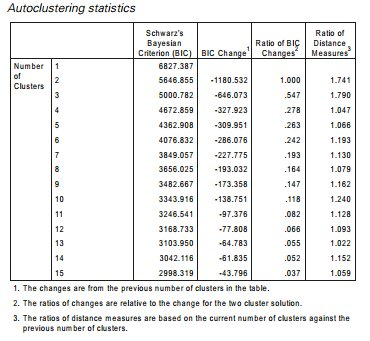
\includegraphics[width=10cm]{TwoStep1.jpg}\\
%  \caption{Schwarz Bayesian Information Criterion}
%\end{centering}
%\end{figure}




\end{document}